\chapter{Développement}

\section{Modifications du framework}

Afin de pouvoir définir des tailles de sprite différentes et rectangulaires, nous avons créé notre propre classe OctolinkSpriteManager. Cela nous a également permi de créer des bounding box avec des tailles personnalisées et de bien les aligner par rapport aux sprites. Nous avons été obligé de dupliquer la classe IntersectTools du framework pour gérer les collisions correctement avec nos bounding box personnalisées.

\begin{figure}[ht!]
  \center
  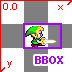
\includegraphics{resources/bbox.png}
  \caption{Link sprite bounding box}
  \label{fig:Link sprite bounding box}
\end{figure}


\section{Architecture du jeu}


\section{Problèmes rencontrés}
